\newcommand\hii{\ion{H}{ii}}

\section{Comparison with observations}
\label{sec:comp-with-observ}


Placing various classes of objects on the \(R_{90}\)--\(R_c\) plane:
\begin{itemize}
\item LL arcs
\item runaway O stars
\item AGB stars
\end{itemize}

\subsection{Mid-infrared arcs around early-type stars}
\label{sec:mid-infrared-arcs}

\begin{figure*}
  \setlength\tabcolsep{0pt}
  \begin{tabular}{ll}
    (a)
    & (b) \\
    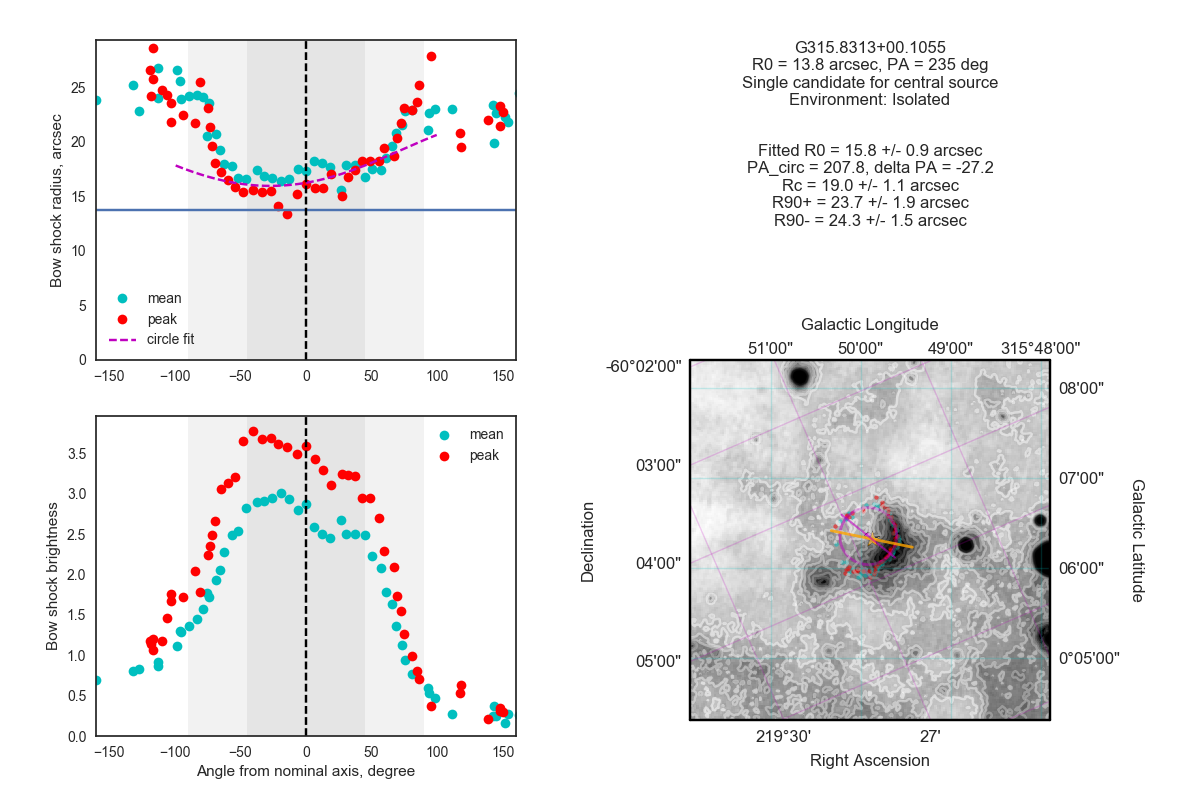
\includegraphics
    [width=0.5\linewidth, trim=20 15 30 10, clip]{figs/0510-3-star}
    & 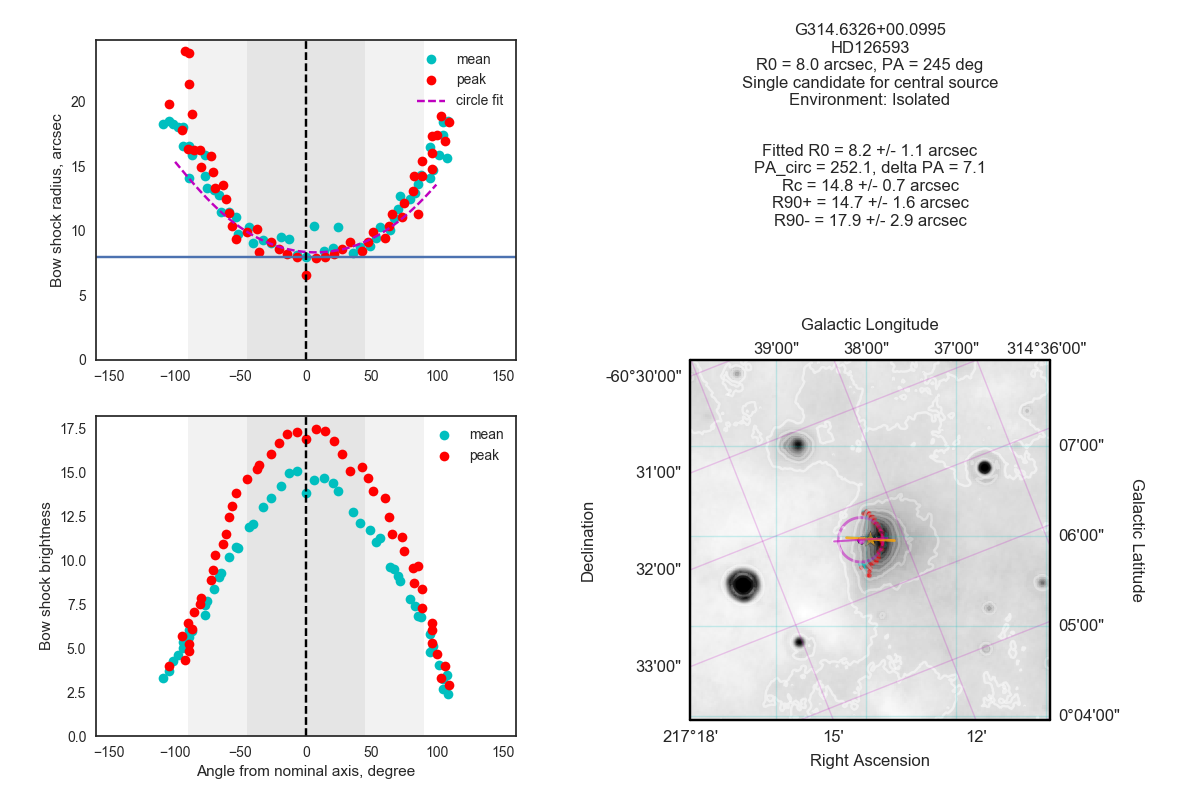
\includegraphics
      [width=0.5\linewidth, trim=20 15 30 10, clip]{figs/0506-4-star} \\
    (c)
    & (d) \\
    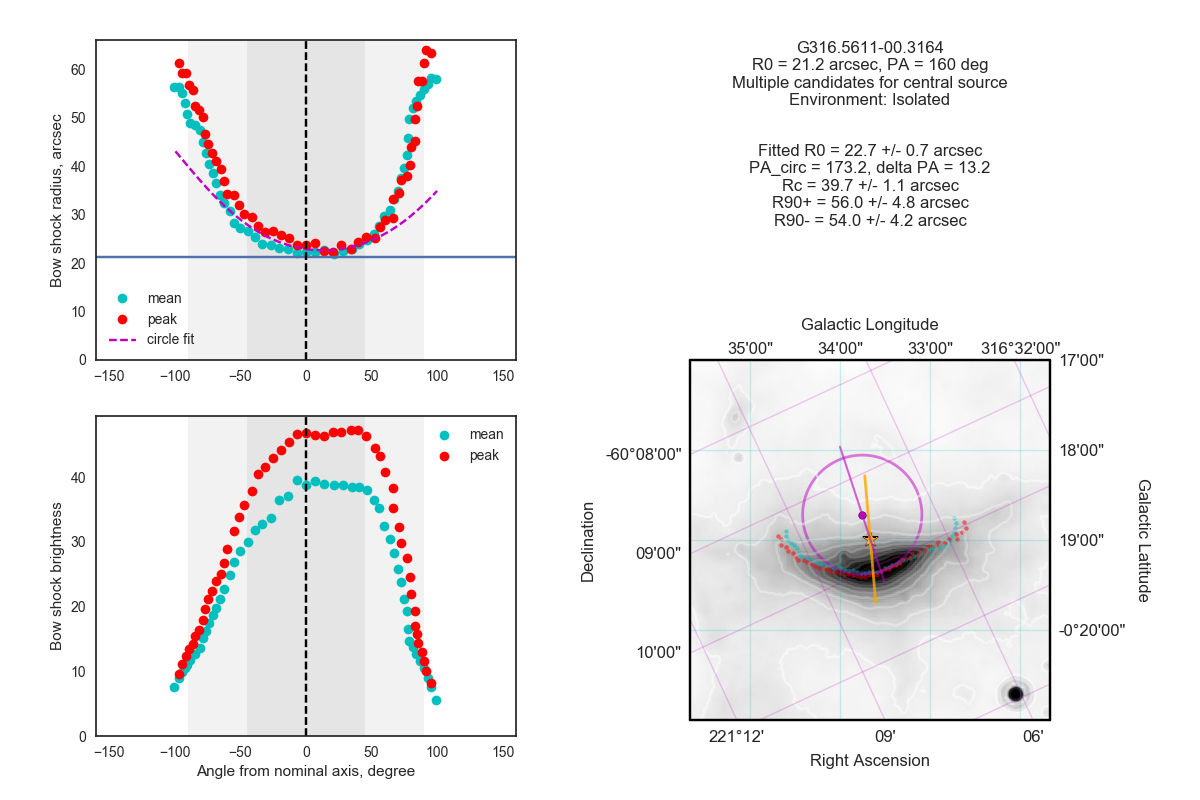
\includegraphics
    [width=0.5\linewidth, trim=20 15 30 10, clip]{figs/0517-5-star}
    & \multicolumn{1}{c}
      {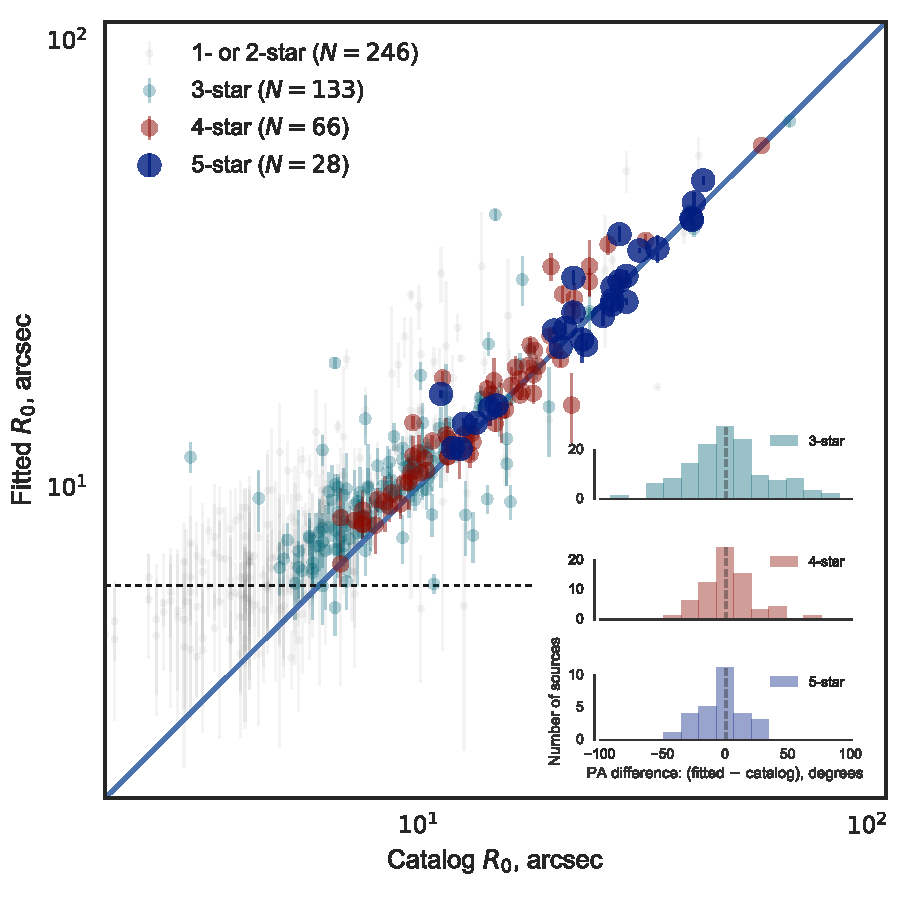
\includegraphics[width=0.35\linewidth, trim=20 20 20 20]
      {figs/mipsgal-r0-r0-plus-dPA-edited}}
  \end{tabular}
  \caption[]{Examples of typical fits to the bow shock shapes of
    MIPSGAL sources with different star ratings: (a) K510, 3-star
    rating; (b) K506, 4-star rating; (c) K517, 5-star rating.  Right
    panels of parts (a)--(c) show a 4\('\) square \SI{24}{\um} image,
    centered on each source.  Contours are ten linearly spaced levels
    between the median brightness of the entire image and the maximum
    brightness of the bow shock arc. Grids of galactic coordinates
    (light blue lines, parallel to the box sides) and equatorial
    coordinates (tilted magenta lines) are shown.  The stellar source
    and the bow shock axis, as determined by \citet{Kobulnicky:2016a}
    are indicated by an orange star and an orange line, respectively,
    where the line extends from \(-2 R_0\) to \(+2 R_0\).  The
    automatically traced arc shapes using the ``mean'' and ``peak''
    methods (see text) are shown by blue and red dots, respectively.
    The magenta circle shows the fit to the arc points within
    \(\pm 45^\circ\) of the nominal bowshock axis, with the magenta dot
    showing the center of curvature and the magenta line showing the
    fitted bow shock axis, which is the line passing through the
    source and the center of curvature.  Left panels of parts (a)--(c)
    show the radius measured from the source (upper panel) and
    brightness (lower panel) of the arc points, plotted as a function
    of angle \(\theta\) from the nominal bow shock axis, and with the same
    color coding as used on the image. Angular ranges of
    \(\theta = \pm 45\degr\) and \(\pm 90\degr\) are shown by gray shaded
    boxes In the upper panel, the \(R_0\) value tabulated by
    \citet{Kobulnicky:2016a} is shown by a horizontal blue line. (d)
    Comparison of the bow shock sizes (scatter plot) and position
    angles (inset histograms) determined from our fits with those
    tabulated by \citet{Kobulnicky:2016a} for the MIPSGAL sources.
    The horizontal dotted line on the main plot shows the MIPS
    \SI{24}{\um} point spread function FWHM of \(5.5\arcsec\).  The
    standard deviation (s.d.) of the position angle differences is
    shown on each inset histogram.}
  \label{fig:mipsgal-examples}
\end{figure*}


The most extensive observational sample of stellar bow shock nebulae
to date is a catalog of 709 arcs \citep{Kobulnicky:2016a} detected in
mid-infrared surveys of the Galactic Plane by the \textit{Spitzer
  Space Telescope} (\textit{SST}, \citealp{Werner:2004a}) and
\textit{Wide-field Infrared Survey Explorer} (\textit{WISE},
\citealp{Wright:2010a}).  These sources are believed to be powered by
the winds of early-type stars, which are either moving supersonically
through the interstellar medium (runaway stars,
\citealp{Gvaramadze:2008a}), or are interacting with a local bulk
flow, such as the champagne flow from a nearby \hii{} region (weather
vanes, \citealp{Povich:2008a}).


\subsubsection{Automatic tracing and fitting of bow shocks}
\label{sec:autom-trac-fitt}


In order to study the shapes of these bow shocks, we downloaded data
from the NASA/IPAC Infrared Science Archive archive\footnote{
  \url{http://irsa.ipac.caltech.edu/docs/program_interface/api_images.html}}
and extracted 4\arcmin{} square images in the \SI{24}{\um} bandpass of
the Multiband Imaging Photometer for \textit{Spitzer} (MIPS) centered
on each of the 471 \citet{Kobulnicky:2016a} sources that are covered
by the MIPSGAL \citep{Carey:2009a} survey, which includes most of the
sources with Galactic longitude within \(\pm 60\degr\) of the Galactic
center.

We developed a methodology for automatically tracing the arcs as follows:
\begin{enumerate}[1.]
\item Calculate arrays of celestial coordinates, \(C\), for each pixel
  of the image.
\item Using the central source coordinates, \(C_0\) and nominal
  bowshock radius, \(R_0\) from \citet{Kobulnicky:2016a}, construct a
  pixel mask that includes only those pixels with separations from the
  source that satisfy \(\frac12 R_0 \le |C - C_0| \le 3 R_0\).  This mask
  will be used for all subsequent operations, which serves to help
  avoid confusion from the star itself and other bright sources in the
  field of view.
\item Define a ``step-back'' point, \(C_1\), which is located at a
  separation \(2 R_0\) from the source, but in the opposite direction
  from the apex of the bow shock. That is, along a position angle
  180\degr{} from the nominal position angle, \(\text{PA}_0\), of the
  bow shock axis.  This point is at one end of the orange line shown
  superimposed on the bow shock images in
  Figure~\ref{fig:mipsgal-examples}.
\item Looping over a grid of 50 position angles, \(\text{PA}_k\),
  within \(\pm 60\degr\) of \(\text{PA}_0\), estimate the location of
  the arc along rays cast from the step-back point, using two
  different methods:
  \begin{enumerate}[(a)]
  \item The pixel with the peak brightness, with coordinates
    \(C_{k,\text{peak}}\) (red dots in
    Fig.~\ref{fig:mipsgal-examples}).
  \item The mean brightness-weighted separation from \(C_1\), with
    coordinates \(C_{k,\text{mean}}\) (light blue dots in
    Fig.~\ref{fig:mipsgal-examples}).
  \end{enumerate}
  For each \(\text{PA}_k\) in the grid, the calculation is performed
  over only those pixels that satisfy
  \(|\text{PA}(C, C_1) - \text{PA}_k| < \frac12 \delta\theta\), where
  \(\delta\theta = 120/50 = 2.4\degr\), which defines a thin radial wedge from
  \(C_1\).  The results are shown as red and blue dots superimposed
  on the images in Figure~\ref{fig:mipsgal-examples}. Each of the two
  methods, ``peak'' and ``mean'', works better in some objects and
  worse in others (according to the subjective judgment of
  ``correctly'' tracing the bow shock shape).  We therefore take the
  average by amalgamating all the \(C_{k,\text{peak}}\) and
  \(C_{k,\text{mean}}\) points into a single set, \(C_{k}\), for
  the following steps.
\item For each of the points \(C_{k}\), determine the radial
  separation from the central source, \(R_k = |C_k - C_0|\) and the
  angle from the bow shock axis about the central source
  \(\theta_k = \text{PA}(C_k, C_0) - \text{PA}_0\).  These are plotted in
  the upper left panels of Figure~\ref{fig:mipsgal-examples}.  Note
  that, even though the rays are cast from the step-back point \(C_1\)
  within \(\pm 60\degr\) of \(\text{PA}_0\), the angles \(\theta_k\) are
  measured from the source, \(C_0\), which is closer to the bow shock
  than \(C_1\) and therefore \(|\theta_k|\) can be much larger than
  \(60\degr\).
\item Make our own estimate of the axial size, \(R_0\), of the bow
  shock by calculating the mean and standard deviation of \(R_k\) over
  all points \(C_k\) with \(|\theta_k| \le 10\degr\).  Note that this is
  distinct from the nominal value of \(R_0\) given in the
  \citet{Kobulnicky:2016a} catalog, which was ``measured by eye''.
\item Estimate the radius of curvature, \(R_c\), by fitting a circle
  to all those points within \(\pm 45\degr\) of the nominal axis
  (\(|\theta_k| < 45\degr\)), but after excluding any point with
  \(R_k < \frac12 R_m\) or \(R_k > 2 R_m\), where \(R_m\) is the median
  \(R_k\) for \(|\theta_k| < 45\degr\).
\item Determine two separate estimates, \(R_{90+}\) and \(R_{90-}\),
  of the perpendicular radius, \(R_{90}\), by taking the mean and
  standard deviation of \(R_k\) over all points \(C_k\) with
  \(|\theta_k - 90\degr| \le 10\degr\) for \(R_{90+}\), and with
  \(|\theta_k + 90\degr| \le 10\degr\) for \(R_{90-}\).
\end{enumerate}


\subsubsection{Subjective evaluation of the fit quality}
\label{sec:subj-eval-fit}


After these automatic steps, we subjectively evaluate the results by giving a star rating to each source:

\paragraph*{0 stars} The fitting algorithm failed for some reason. 

\paragraph*{1 star} The fit was formally successful, but the results
for \(R_c\) or \(R_{90}\) are far removed from what a human would
predict by looking at the image.  For example, in the smallest
bowshocks, which are only marginally resolved by Spitzer's 6\arcsec{}
beam, the dispersion in \(R_k\) can be a significant fraction of
\(R_0\), in which case our algorithm tends to erroneously favor
\(R_c < R_0\).

\paragraph*{2 stars} The fit results are not totally outlandish, but
nonetheless some problem is apparent that casts doubt on their
reliability.  For example, a double-shell structure to the bow shock
that leads to large differences between the ``peak'' and ``mean''
methods, or point sources near to the bow shock that interfere with
the tracing procedure.
  
\paragraph*{3 stars} A good fit, but where the dispersion in \(R_k\)
and/or the asymmetry in the bow shock reduces the precision in the
determination of \(R_c\) and \(R_{90}\), giving subjectively estimated
uncertainties around the 20\% level.  An example of a 3-star fit is
shown in Figure~\ref{fig:mipsgal-examples}a.

\paragraph*{4 stars} A high quality fit, with subjectively estimated
uncertainties in \(R_c\) and \(R_{90}\) around the 10\% level. An
example of a 4-star fit is shown in
Figure~\ref{fig:mipsgal-examples}b.

\paragraph*{5 stars} The highest-quality fit, usually corresponding to
large, sharply defined bow shocks, whose shape is determined with high
precision. An example of a 5-star fit is shown in
Figure~\ref{fig:mipsgal-examples}c.

\bigskip
%
Figure~\ref{fig:mipsgal-examples}d compares the bow shock size,
\(R_0\), determined by our fits (vertical axis) with the corresponding
value given in the \citet{Kobulnicky:2016a} catalog (horizontal axis).
For most sources with 3-star or higher rating, the two estimates agree
to within \(\pm 20\%\), but there are a small number of sources with a
discrepancy of more than a factor of two.  In all cases that we
checked, we believe that our estimates of \(R_0\) are more accurate
than those in the catalog.  It is apparent that the star ratings are
correlated with the bow shock size, with larger bow shocks tending to
receive higher ratings, although there is considerable overlap.  In
particular, most of the 1- and 2-star sources are close to the
resolution limit of the MIPSGAL \SI{24}{\um} images (\(6\arcsec\),
indicated by the dotted horizontal line in te figure).

\begin{figure*}
  \centering
  \begin{tabular}{ll}
    (a) & (b) \\
    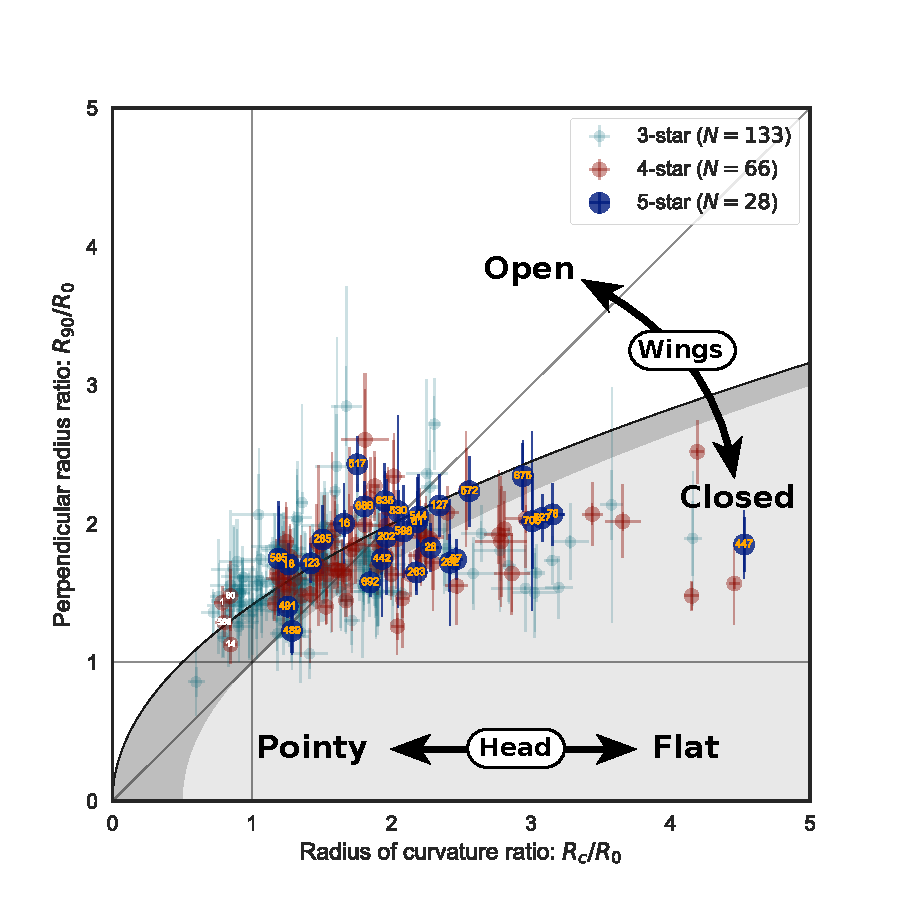
\includegraphics[width=0.45\textwidth, trim=0 0 30 0]
    {figs/mipsgal-Rc-R90-zoom-annotated}
        & 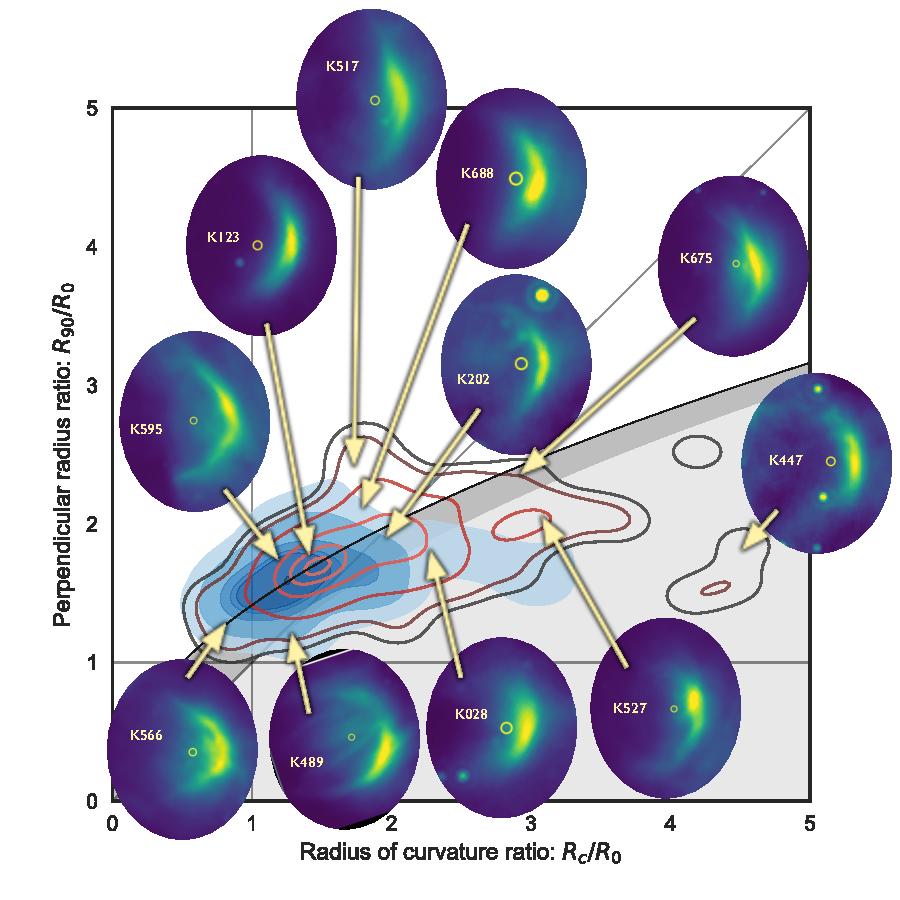
\includegraphics[width=0.45\textwidth, trim=0 0 30 0]
          {figs/mipsgal-Rc-R90-thumbnails} 
  \end{tabular}
  \caption[]{MIPSGAL sources on the bow shock shape diagnostic diagram
    of dimensionless radius of curvature versus perpendicular radius.
    The regions corresponding to different classes of cuadrics are
    shown by shading (see \S~\ref{sec:conic}): oblate spheroids (light
    gray background); prolate spheroids (darker gray background);
    paraboloids (curved black line); hyperboloids (white background).
    (a) Individual sources with bow shock fit quality rating of 3-star
    or above.  All 5-star sources plus those 4-star sources with
    \(R_c/R_0 < 1\) are labelled with their \cite{Kobulnicky:2016a}
    catalog number.  Horizontal error bars do not directly reflect the
    uncertainty in \(R_c/R_0\) but are instead simply the standard
    deviation from the circle fit of bowshock points \(R_k\) within
    \(\pm 45\degr\) of the axis.  Values on the vertical axis
    represent the average of \(R_{90+}\) and \(R_{90-}\), with thin
    vertical error bars showing the difference between \(R_{90+}\) and
    \(R_{90-}\), and thick vertical error bars showing the rms
    dispersion of \(R_k\) about these values for bow shock points
    within \(\pm 10\degr\) of the \(+90\degr\) and \(-90\degr\)
    directions.  (b) Kernel density estimator (KDE) of the
    distribution for 3-star sources (blue, filled contours) and 4-
    plus 5-star sources (orange/brown, unfilled contours).  The KDE
    uses an anisotropic gaussian kernel with bandwidths of
    \(0.18 \times 0.12\). Images of representative 4- and 5-star sources at
    different points on the \(R_c\)--\(R_{90}\) plane are also shown.}
  \label{fig:mipsgal-shapes}
\end{figure*}

In the following analysis, only those sources with a 3-star or higher
rating are used.  These comprise approximately half (227 out of 471)
of all the MIPSGAL arc sources.  In some cases of poor and failed
fits, there is nothing apparently ``wrong'' with the source itself,
and it is likely that minor tweaks to the methodology would improve
matters, but we have elected not to do so, in order to maintain a
uniform methodology across all sources.

The inset of Figure~\ref{fig:mipsgal-examples}d shows histograms of
the difference between the position angle, \(\text{PA}_0\) determined
by our fits and that listed in \citet{Kobulnicky:2016a}.  Although
observational uncertainties undoubtedly contribute in part, the
differences are mainly due to real asymmetries in the bow shocks,
especially for the 4- and 5-star sources.  The
\citeauthor{Kobulnicky:2016a} catalog \(\text{PA}_0\) values are
mostly sensitive to the orientation of the bow shock wings, whereas
our fitted \(\text{PA}_0\) values are determined by the point in the
bow shock head that is closest to the stellar source.  For this
reason, we use the catalog \(\text{PA}_0\) values for defining the
axis when measuring \(R_{90+}\) and \(R_{90-}\). On the other hand,
the fitted values of \(\text{PA}_0\) are better correlated with the
position of the bow shock's brightness peak, as is apparent in the
lower left panels of Figure~\ref{fig:mipsgal-examples}a and c.

\subsubsection{OB bow shock shapes on the diagnostic plane}
\label{sec:ob-shapes}

The derived bowshock shapes of all the 3-, 4-, and 5-star sources are
shown in Figure~\ref{fig:mipsgal-shapes} on the plane of \(R_c/R_0\)
versus \(R_{90} / R_0\).  Panel a shows the individual points
superimposed on the theoretical results for quadrics of revolution
(see figure caption and \S~\ref{sec:conic}), while panel b shows
contours of the kernel density estimator (KDE, see
\citealp{Leiva-Murillo:2012a, Scott:2015a}) of the two-dimensional
distribution of points on the \(R_c\)--\(R_{90}\) plane.  The
horizontal axis corresponds to the shape of the head of the bow shock
near its apex, ranging from sharper, pointier shapes with
\(R_c/R_0 < 1\) to flatter, snubber shapes with \(R_c/R_0 \gg 1\), where
it must be understood that all judgments of sharpness/flatness are
with respect to the axial separation, \(R_0\), between the source and
the bow shock apex.  The vertical axis corresponds to the shape of the
bow shock wings, ranging from closed ``C'' shapes for smaller values
of \(R_{90} / R_0\) to open ``V'' shapes for larger values of
\(R_{90} / R_0\).  The boundary between closed and open corresponds to
the paraboloids, and is shown by the solid curved line that divides
the shaded from the unshaded regions of the graph.

The KDE contours in Figure~\ref{fig:mipsgal-shapes}b show that the
distribution of 3-star sources is very similar to that of 4- and
5-star sources, although the higher-rated sources are shifted slightly
to the upper right.  This is probably due to higher-rated sources
being on average bigger, as will be discussed further below.  The bulk
of the sources are concentrated around the paraboloid line, with
\(1 < R_c/R_0 < 2.5\), and \(1.2 < R_{90}/R_0 < 2\).  But significant
minorities are found in three other regions: (1)~a clump with
\(R_c/R_0 \la 1\); (2)~a vertical spur towards higher \(R_{90}\) at
\(R_c/R_0 \approx 2\); and (3)~a broad horizontal tail towards higher
\(R_c\) at \(R_{90}/R_0 \la 2\).


\subsubsection{Correlation between bow shock size and other parameters}
\label{sec:corr-size}

\begin{figure*}
  \centering
  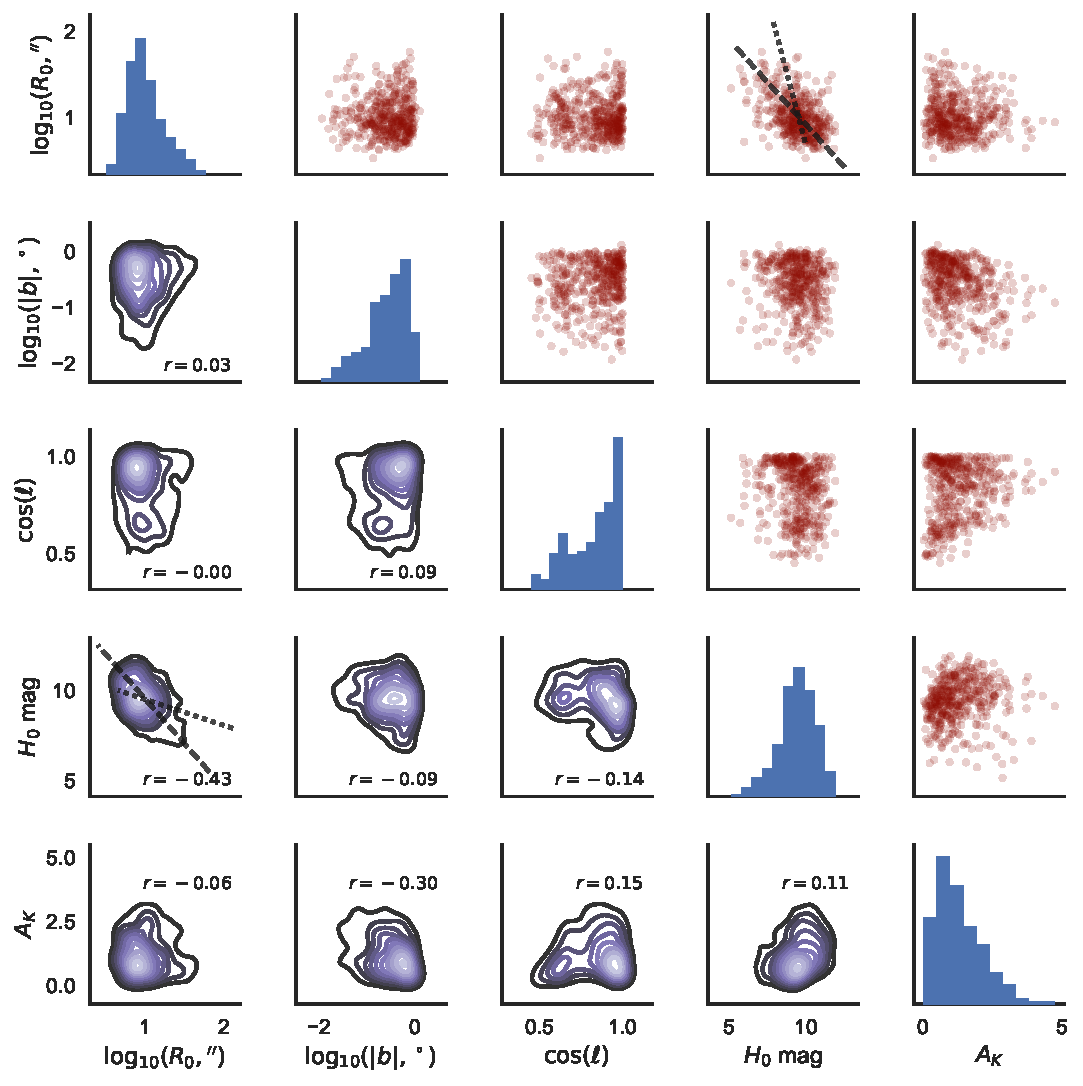
\includegraphics[width=0.8\textwidth]{figs/mipsgal-pairplot}
  \caption[]{Matrix of pair plots that illustrate distributions of and
    correlations between the non-shape parameters of all MIPSGAL bow
    shock sources from \citet{Kobulnicky:2016a}.  Plots on the leading
    diagonal show histograms of the following parameters: bow shock
    angular size, \(\log_{10} R_0\); Galactic latitude,
    \(\log_{10}|b|\); Galactic longitude, \(\cos \ell\);
    extinction-corrected \(H\)-band magnitude of the stellar source,
    \(H_0\); \(K\)-band extinction, \(A_K\).  Scatter plots in the
    upper triangle show the joint distribution of each pair of
    parameters.  These are repeated in the lower triangle but showing
    the KDEs of the joint distributions, which are annotated with the
    Pearson linear correlation coefficient, \(r\), for each pair. The
    straight lines shown superimposed on the plots of stellar magnitude
    versus bowshock size correspond to toy model results for the same star
    at a sequence of distances (dashed lines) and a sequence of
    stellar luminosities at a fixed distance (dotted lines).  See text
    for details. }
  \label{fig:mipsgal-pairplot}
\end{figure*}

In Figure~\ref{fig:mipsgal-pairplot} we show the distributions over
all MIPSGAL bow shock sources of the bow shock size, Galactic
coordinates, extinction-corrected stellar source magnitude, and dust
extinction.  For the bow shock size, \(R_0\), we use the results from
our model fitting rather than the values given in the
\citet{Kobulnicky:2016a} catalog, but the distribution is very
similar, as can be seen by comparing the top-left plot of
Figure~\ref{fig:mipsgal-pairplot} with \citeauthor{Kobulnicky:2016a}'s
Figure~8.

The catalog gives the \(K\)-band extinction, \(A_K\), derived using
the method of \citet{Majewski:2011a}, but that assumes an intrinsic
color of \((H - [\SI{4.5}{\um}])_0 = +0.08\) magnitudes, which is too
red if the sources are assumed to be OB stars.  We therefore re-derive
\(A_K\) from the catalog magnitudes combined with the
\citet{Indebetouw:2005a} reddening law, but assuming
\((H - [\SI{4.5}{\um}])_0 = -0.1\) magnitudes, which is more typical
of early type stars.  This does not make very much difference (compare
the top-right plot of our Fig.~\ref{fig:mipsgal-pairplot} with
\citeauthor{Kobulnicky:2016a}'s Fig.~9), but it does eliminate some of
the apparent negative extinctions that are found in the catalog.  The
same reddening law gives \(A_H = 1.55 A_K\), and this is used to
derive extinction-corrected \(H\)-band apparent magnitudes, \(H_0\).

The most significant linear correlation between any pair of parameters
in Figure~\ref{fig:mipsgal-pairplot} is that between bow shock size
and stellar source brightness: \(H_0\) versus \(\log_{10} R_0\), with
correlation coefficient \(r = -0.43\).  The distribution of \(H_0\)
depends on the absolute magnitude, \(M_H\), and the distance, \(d\),
to the source.  It is likely that variation in \(d\) is the more
important of the two because \(M_H\) changes relatively little for
main-sequence OB stars, ranging from \(M_H \approx -4\) (early-O) to
\(M_H \approx -1.5\) (mid-B).  This is because part of the increase in
bolometric luminosity, \(L\), as one ascends the main sequence is
offset by an increase in the effective temperature,
\(T_{\text{eff}}\), which shifts the peak of the stellar spectrum
farther away from the \(H\)~band, resulting in
\(L_H \propto L / T_{\text{eff}}^3 \sim L^{0.53}\), where the last step uses
the upper main-sequence mass--luminosity and mass--radius scalings from
\citet{Eker:2015a}. It is true that evolved OB supergiants can be much
brighter, reaching \(M_H \approx -7\), but such stars are expected to be
rare.  Assuming a B2V star (\(M_H = -2\)), then the observed range
\(H_0 = 5\)--\(12\) corresponds to distances
\(d = 100\)--\SI{6300}{pc}, and the histogram peak at
\(H_0 \approx 9.5\) corresponds to \(d \approx \SI{2000}{pc}\), which is all
perfectly reasonable.

Turning now to the distribution of bow shock angular size, \(R_0\),
this will also be affected by distance to at least some degree, since
for a constant physical size the angular size will vary as
\(R_0 \propto d^{-1}\).  For instance, if we assume that the physical size
of all bow shocks is \SI{0.1}{pc} and the absolute magnitude of all
stars is \(M_H = -2\), as above, then we find the relation
\(H_0 = 14.57 - 5 \log_{10} R_0\) if \(R_0\) is measured in
arcseconds. This is shown as a dashed line on the relevant panels of
Figure~\ref{fig:mipsgal-pairplot} for values of \(R_0\) that
correspond to \(d = \SI{300}{pc}\) to \SI{8000}{pc}.  It can be seen
that this relation is in excellent agreement with the linear trend in
the data. On the other hand, the correlation coefficient of
\(r = -0.43\) means in broad terms that only a fraction
\(r^2 \approx 20\%\) of the total variance in \(H_0\) is ``explained'' by
changes in \(R_0\), and vice~versa, implying that one or both of
\(H_0\) and \(R_0\) is only a very imperfect proxy for \(d\).  We have
already seen that the spread in \(H_0\) probably \emph{is} mostly due
to a spread in distance, rather than a spread in \(H\)-band stellar
luminosity.  If this is true, it follows that it is \(R_0\) that
depends only weakly on \(d\) and is more influenced by other factors.

\begin{figure*}
  \centering
  \begin{tabular}{ll}
    (a) & (b) \\
    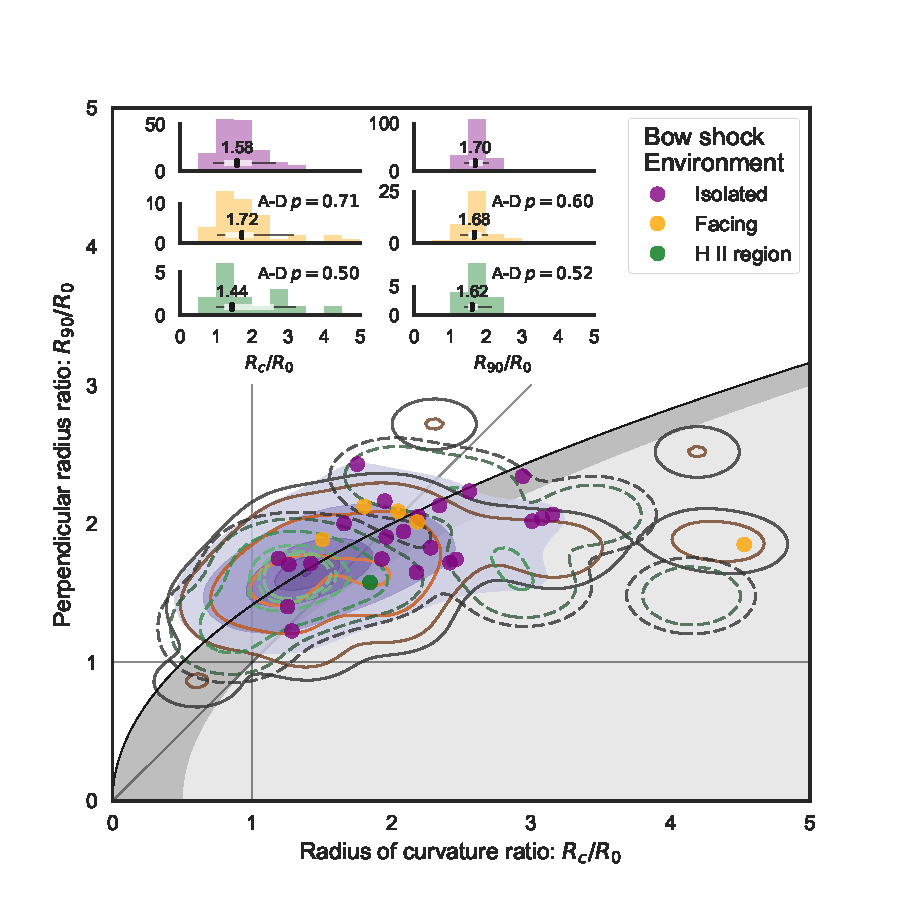
\includegraphics[width=0.45\textwidth]{figs/mipsgal-Rc-R90-environment} &
    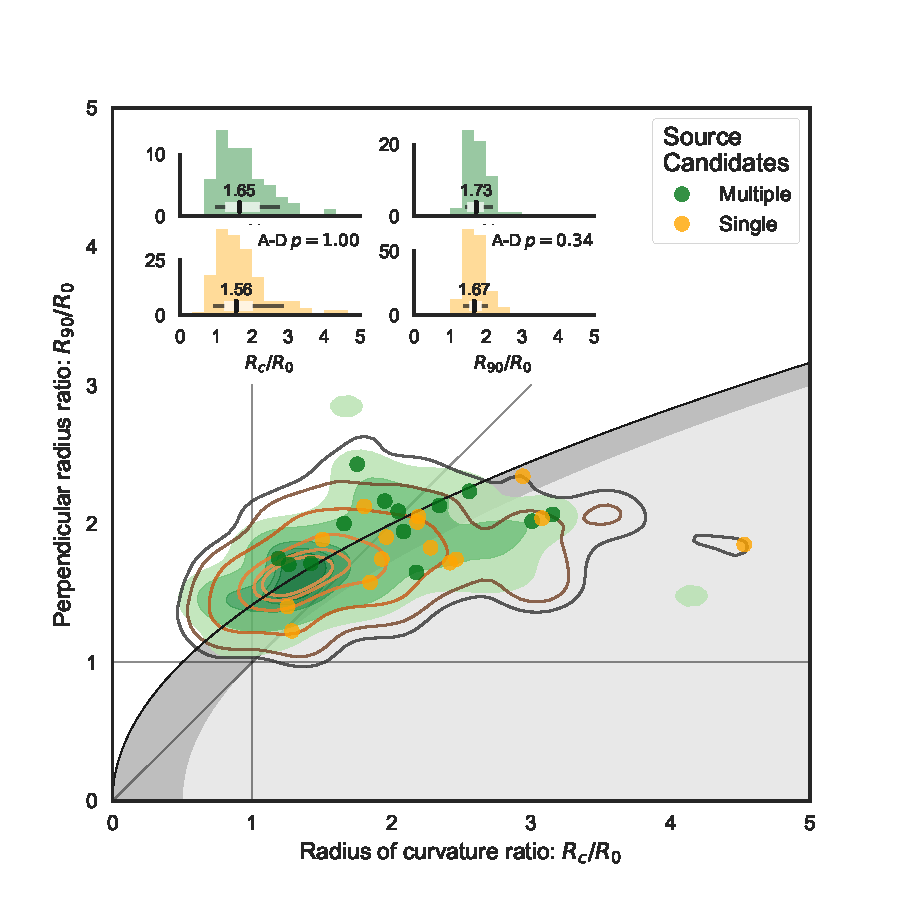
\includegraphics[width=0.45\textwidth]{figs/mipsgal-Rc-R90-candidates} 
  \end{tabular}
  \caption[]{Lack of significant correlation of bow shock shape with
    (a) environment, and (b) uncertainty in stellar source
    identification.}
  \label{fig:mipsgal-uncorrelated}
\end{figure*}

One such factor is the stellar/environmental momentum-loss ratio,
\(\beta\), between the two supersonic flows that form the bow shock.  All
other things being equal, we have \(R_0 \propto \beta^{1/2}\) for
\(\beta \ll 1\), as is typically the case.  If the environment flow is
constant and the OB star wind has mass-loss rate \(\dot{M}\) and
terminal velocity \(V_\infty\), then
\(\beta \propto \dot{M}{V_\infty}\).  Empirical and theoretical studies of hot star
winds (e.g., \citealp{Puls:1996a}) imply
\(\dot{M}{V_\infty} \sim L^{1.88} R^{-1/2} \sim L^{1.80} \sim L_H^{3.40}\), where
the final two steps apply only to main-sequence stars and again use
the relations of \citet{Eker:2015a}.  If we assume as above that a B2V
star with \(M_H = -2\) has a bow shock physical size of \SI{0.1}{pc},
and consider a sequence of stars with varying \(H\)-band luminosities
but all at a fixed distance of \(d = \SI{2000}{pc}\), then we find the
relation \(H_0 = 8.02 - 1.49 \log_{10} R_0\).  This is shown as a
dotted line in the relevant panels of
Figure~\ref{fig:mipsgal-pairplot} for the absolute magnitude range
\(M_H = -3.6\) (O6V) to \(M_H = -1.5\) (B5V).  It can be seen that
this relation does not match the linear trend in the data, and
predicts a much larger spread in \(R_0\) over a narrow range in
\(H_0\) than is observed.  This could mean one of two things: first,
it may be that the range of stellar luminosities is significantly
narrower than we have supposed, implying that B stars vastly outnumber
O stars among the sources.  Alternatively, there may be a positive
correlation between the stellar luminosity and the momentum of the
environmental flow, with the result that \(\beta\) varies less steeply
with \(L_H\) than we have assumed.  That could arise if more luminous
stars were preferentially found in denser environments, or, in the
case of runaways, if more luminous stars tended to be faster moving.

A third factor that may influence \(R_0\) is the inclination, \(i\),
of the bow shock axis with respect to the plane of the sky.
Figure~\ref{fig:quadric-projection}b shows that for \(R_c > 1\), then
the projected \(R_0'\) becomes larger than the true \(R_0\) as \(|i|\)
increases.  This is further illustrated in
Figure~\ref{fig:projected-R90-Rc-snapshots} for simple quadric shapes
(spheroids, paraboloids, hyperboloids) and in
Figure~\ref{fig:thin-shell-R90-Rc-snapshots} for the carawilkinoids
and ancarawilkinoids.  It can be seen that the effect is relatively
modest for bow shocks with projected shapes falling in the range
\(1 < R_c/R_0 < 3\) and \(R_{90}/R_0 < 3\), as the vast majority of
our observed sources do.  The increase in \(R_0\) is no more than a
factor of 2 to 3 for moderate inclinations of \(30\) to \(60\degr\),
although it can reach a factor of 5 to 10 for some shapes at more
extreme inclinations.

%% Maybe talk about the other correlations later if we have time

\subsubsection{Correlation between bow shock shape and other parameters}
\label{sec:corr-shape}
\begin{figure*}
  \centering
  \begin{tabular}{ll}
    (a) & (b) \\
    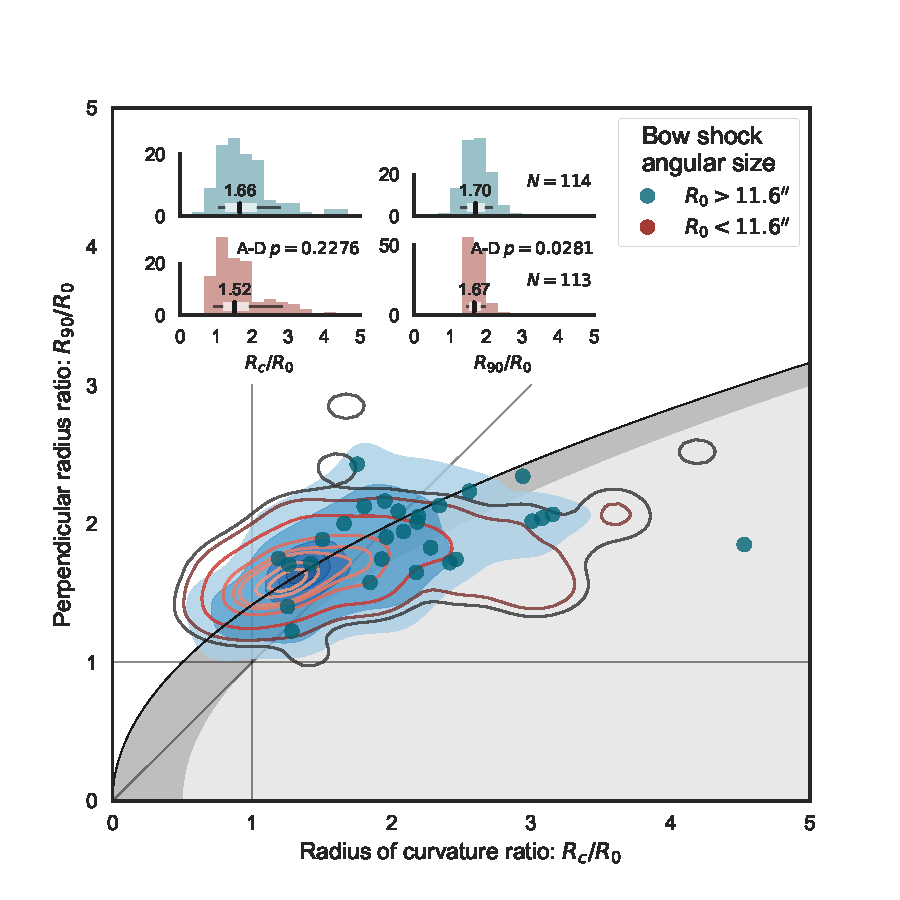
\includegraphics[width=0.45\textwidth]{figs/mipsgal-Rc-R90-R0} &
    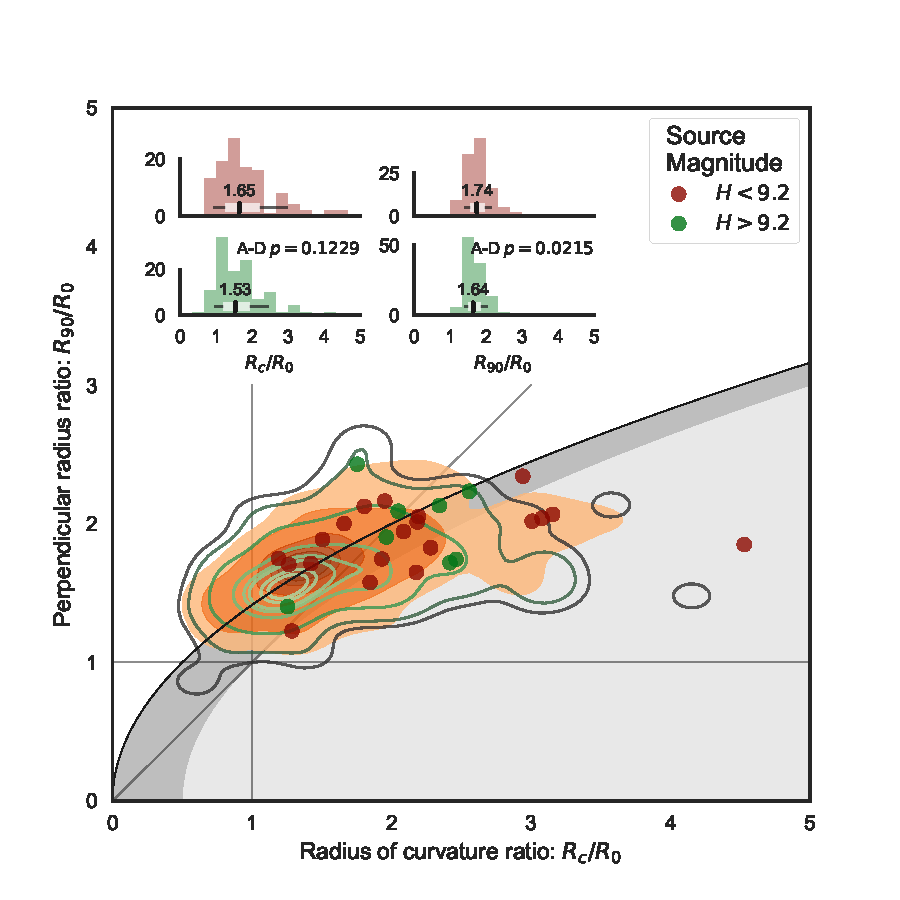
\includegraphics[width=0.45\textwidth]{figs/mipsgal-Rc-R90-Mag} 
  \end{tabular}
  \caption[]{Comparison between the distribution of bowshock shapes
    when the sources are divided into two sub-samples according to the
    value of another parameter. (a)~Bow shock angular size, \(R_0\).
    (b)~Extinction-corrected \(H\)-band magnitude of the stellar
    source.}
  \label{fig:mipsgal-correlated}
\end{figure*}

\begin{figure}
  \centering
  \setlength\tabcolsep{0pt}
  \begin{tabular}{ll}
    (a) & (b) \\
    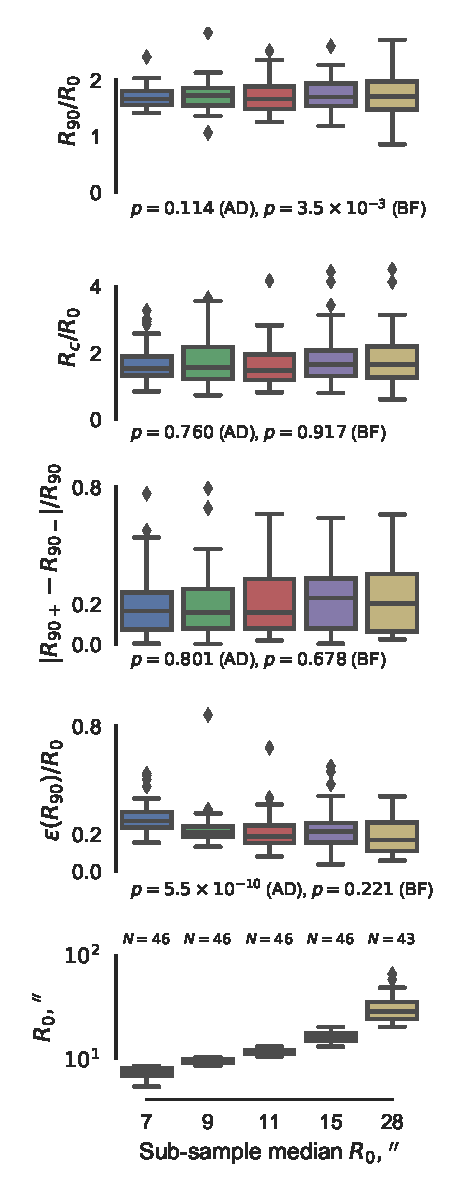
\includegraphics[height=1.167\linewidth]{figs/mipsgal-boxplot-Rc-R90-versus-R0}
    & 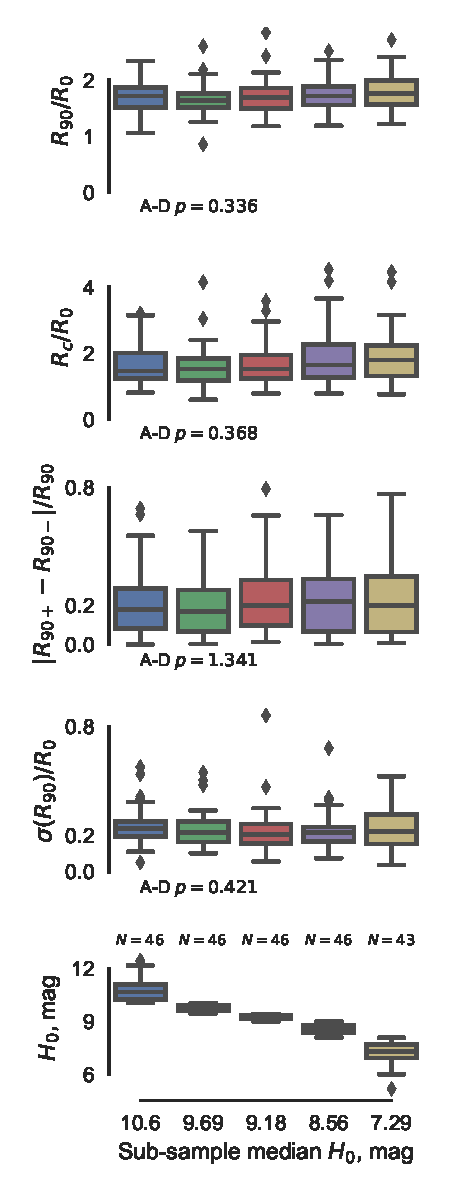
\includegraphics[height=1.167\linewidth]{figs/mipsgal-boxplot-Rc-R90-versus-H0}
  \end{tabular}
  \caption{(a) Box plots of the distributions of bow shock shape
    parameters, \(R_c/R_0\) and \(R_{90} / R_0\), together with a
    measure of the tail asymmetry, \(|R_{90+} - R_{90-}| / R_{90}\),
    after partitioning on the bow shock size, \(R_0\).  All 3-, 4-,
    and 5-star sources are sorted according to \(R_0\) and divided
    into 5 non-overlapping sub-samples of roughly equal size, each
    labelled by their median value of \(R_0\) in arcseconds, as
    illustrated in the lower panel.  The colored boxes show the
    interquartile range, with the median indicated by a horizontal
    line, the 1st-to-9th interdecile range by error bars, and outliers
    by diamonds.  A 5-sample Anderson--Darling test is performed for
    each dependent variable, with resultant \(p\)-value given at the
    bottom of each panel.  It is apparent that the dispersion in
    \(R_{90} / R_0\) (upper panel) increases systematically with
    \(R_0\), although the central value is roughly constant.  No clear
    systematic changes are apparent in \(R_c / R_{90}\) (middle
    panel).  (b)~As (a), but partitioning on the extinction-corrected
    \(H\)-band magnitude, \(H_0\).  Note that sub-samples are plotted
    in order of \textit{decreasing} magnitude to allow comparison
    between (a) and (b), given the negative correlation between
    \(H_0\) and \(R_0\) (see Fig.~\ref{fig:mipsgal-pairplot}).}
  \label{fig:mipsgal-boxplot}
\end{figure}

We now investigate if the bow shock shapes of the MIPSGAL sources are
correlated with any other parameters via the following methodology:
\begin{enumerate}[1.]
\item For each of the parameters in the \citet{Kobulnicky:2016a}
  catalog, we divide the sources into two or more sub-samples,
  according to the value of the parameter.  For quantitative
  parameters, such as those discussed in the previous section, we use
  two sub-samples of equal size, with membership determined by whether
  the parameter is larger or smaller than the median value.  But we
  also use categorical parameters, such as the type of bow shock
  environment, or the presence/absence of \SI{8}{\um} emission, in
  which case the sub-samples are of unequal size.
\item We plot the KDEs of the two sub-samples separately on the
  \(R_c\)--\(R_{90}\) plane (see Figs.~\ref{fig:mipsgal-correlated} and
  \ref{fig:mipsgal-uncorrelated}) to check for any obvious
  differences.
\item We test if there is any statistically significant difference
  between the bow shock shapes of the sub-samples by applying the
  two-sample Anderson--Darling test \citep{Anderson:1952a,
    Scholz:1987a, Makarov:2017a} to \(R_c/R_0\) and \(R_{90}/R_0\)
  separately.  This is a non-parametric test of the \textit{null
    hypothesis} that the two sub-samples are drawn from the same
  distribution.  It returns a \(p\)-value, which is the estimated
  probability that the observed difference between the two sub-samples
  would be as large as it is purely by chance if they were all were
  drawn from the same distribution.  We adopt a threshold of
  \(p < 0.001\) in order to confidently reject the null hypothesis and
  declare a ``significant'' difference between the two sub-samples,
  but we also consider the less strict threshold of \(p < 0.05\) as an
  indicator of ``probable'' difference (see
  Appendix~\ref{sec:distr-p-values} for details).
\end{enumerate}

\subsection{Far-infrared arcs around late-type stars}
\label{sec:far-infrared-arcs}

\begin{figure}
  \centering
  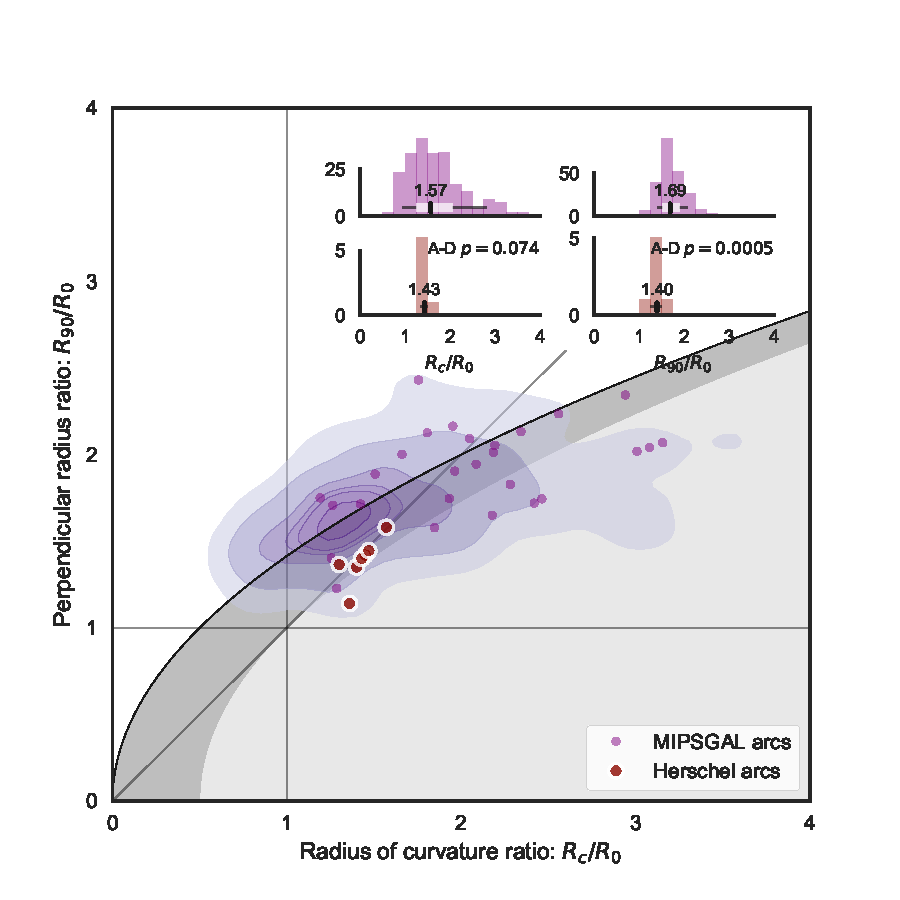
\includegraphics[width=\linewidth]{figs/mipsgal-Rc-R90-vs-Herschel}
  \caption[]{Comparison of RSG/AGB arcs with OB star arcs.}
  \label{fig:herschel-compare-mipsgal}
\end{figure}



\subsection{Stationary emission line arcs in M42}
\label{sec:stat-emiss-line}

\begin{figure*}
  \centering
  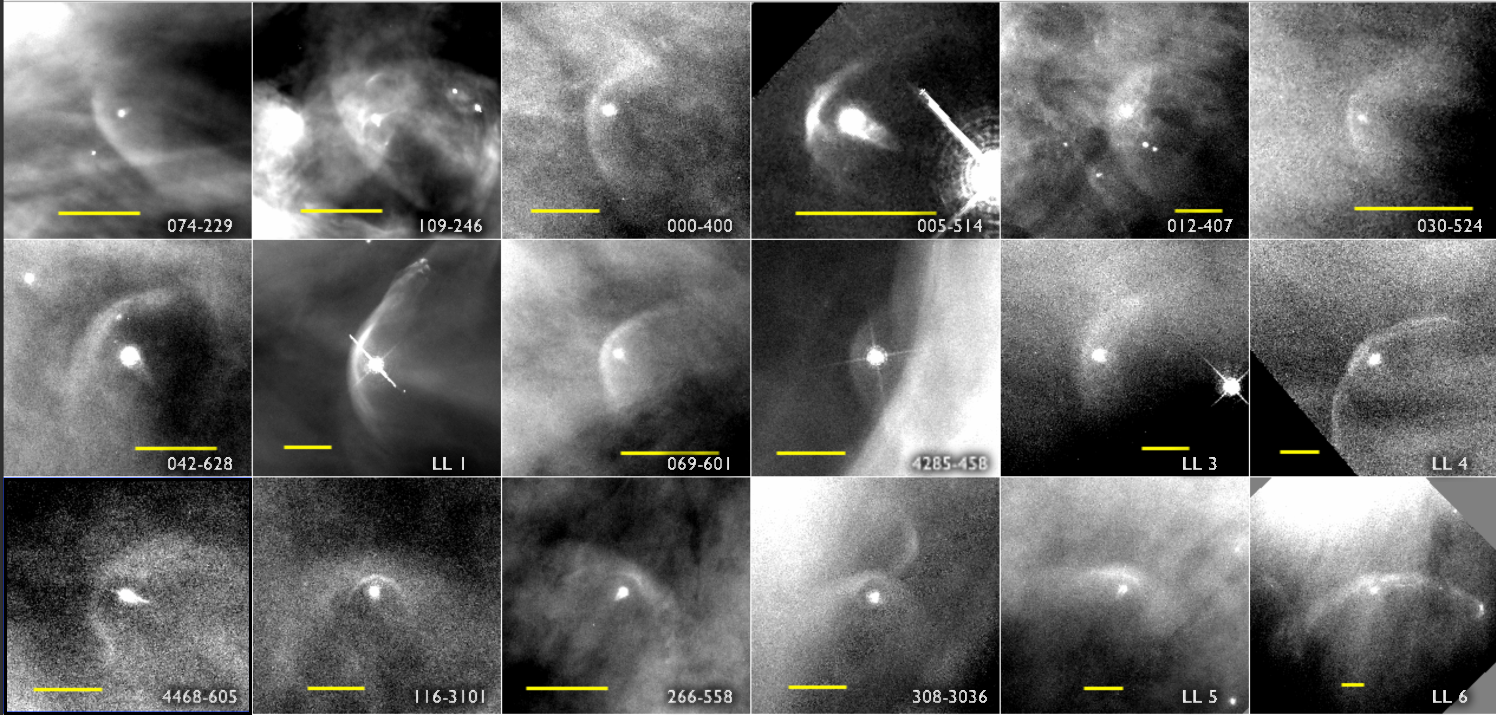
\includegraphics[width=\textwidth]{figs/annotated-ll-arcs}
  \caption[]{Stationary bow shock arcs in the Orion Nebula.}
  \label{fig:ll-arcs}
\end{figure*}

\begin{figure}
  \centering
  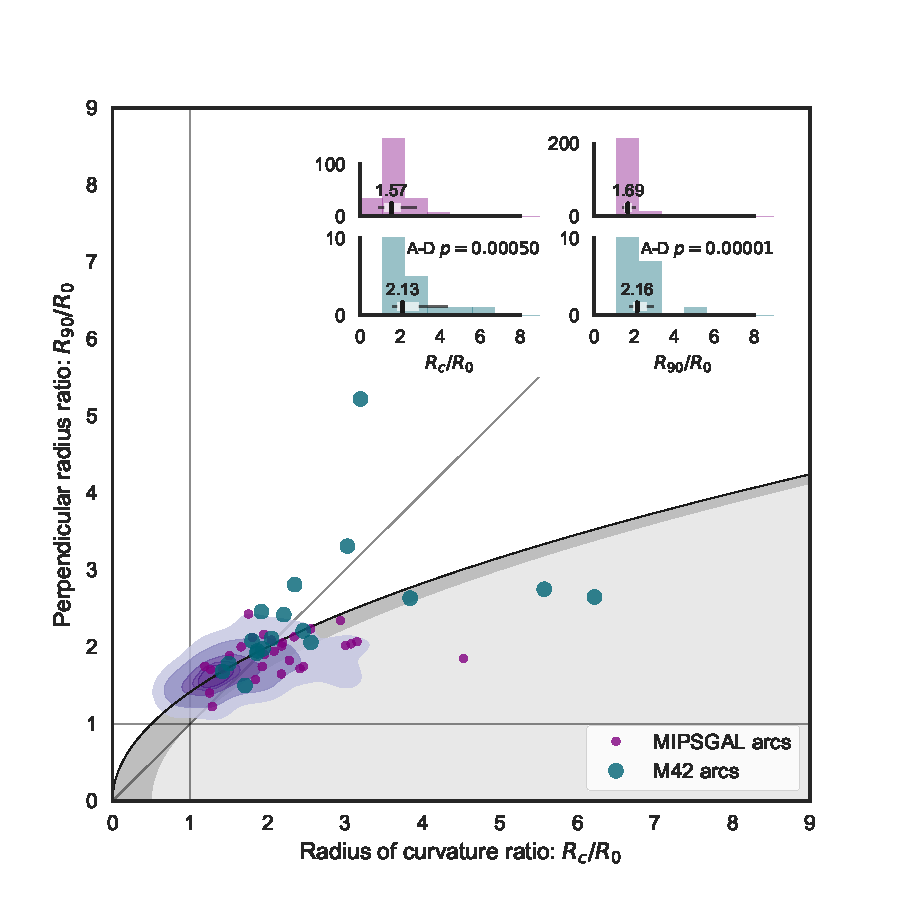
\includegraphics[width=\linewidth]{figs/mipsgal-Rc-R90-vs-Orion}
  \caption[]{Comparison of Orion with OB stars.}
  \label{fig:ll-compare-mipsgal}
\end{figure}


Mention future JWST observations with \(0.85\arcsec\) resolution at \SI{22}{\um}. 


%%% Local Variables:
%%% mode: latex
%%% TeX-master: "quadrics-bowshock.tex"
%%% End:
